% !TEX root =  ../report.tex
% !TeX spellcheck = en-GB

\section{Introduction}
%The introduction should provide content for the report, discuss relevant background material and state the main aims of the work. Clearly establishing the aims of the work is important for this coursework, since you have a great deal of freedom in what you will seek to achieve.

In the field of High Performance Computing (HPC), computers with processing power hundreds of times greater than conventionally available machines are used to solve or approximate complex problems. Such computers have been required for some time to utilise parallelism, in order to find solutions within a reasonable run-time.
\par Many paradigms for executing parallel workloads have emerged over time. Recently, General Purpose Graphical Processing Units (GPUs) have become an increasingly popular hardware architecture, having originally been conceived as specialised hardware for graphical shader calculations. GPU's high number of parallel processing units allow a high degree of parallelism, as well as being able to execute operations usually done by the CPU. Passing compute-heavy workloads to a GPU device can provide very significant speed-up over sequential execution, and remove the CPU as a bottleneck.
\par
Commonly, a single developer or team is unlikely to have both the necessary expertise in a niche area of physics with a non-trivial problem to be solved; and also sufficient depth of knowledge in computer science to understand the latest generation of parallel hardware. For this reason the OP2 framework was created: to provide a high level abstraction in which HPC applications can be written, and separate the application code from the optimisation requirements. OP2 is already able to generate optimised code for a number of back-ends from an application file.
\par
This report details an investigation into implementing and benchmarking a new optimisation to the GPU code generation in OP2. The optimisation is named ``Just-In-Time Compilation" for its similarities to a comparable process often performed by compilers when run-time efficiency is desired.
\vfill
\subsection{Motivations}
The idea for this project was provided by my supervisor, Dr Gihan Mudalige - an Associate Professor in the University of Warwick Computer Science Department. It was pulled from the pool of uncompleted features for the OP2 project, and was selected because it aligned with my interest in High Performance Computing, and previous experience with optimising existing codes.
\par
Since OP2 is Open Source and freely available, the implementation I produce will become part of the framework, allowing future contributors to build on my work.

\subsection{Background Work}
\label{s:bgwork}

In order to become comfortable with the OP2 framework and provide a useful contribution, it is important to understand the domain of problems for which it was created: Unstructured Mesh Solvers.
\par
A large proportion of HPC workloads involve approximating Partial Differential Equations (PDEs) to simulate complex interactions in physics problems, for example the Navier-Stokes equations for computational fluid dynamics, or predicting weather patterns. It is usually necessary to discretise such problems, which means dividing a continuous space into a number of discrete cells such as in Figure \ref{fig:2dmesh}.
\begin{figure}[h!]
  \begin{minipage}{.5\textwidth}
    \centering
    \begin{tikzpicture}[x=2.6ex, y=2.6ex]
      \draw (0,6) -- (0,3) -- (5,3) -- (5,0) -- (8,0) -- (8,2) -- (9,2) -- (9,6) -- (8,6) -- (8,7) -- (4,7) -- (4,6) -- cycle ;
    \end{tikzpicture}
  \end{minipage}
\begin{minipage}{.5\textwidth}
  \centering
  \begin{tikzpicture}
  \tikzset{
    square matrix/.style={
      matrix of nodes,
      column sep=-\pgflinewidth, row sep=-\pgflinewidth,
      nodes={
        rectangle,
        draw=black,
        minimum height=#1,
        anchor=center,
        align=center,
        text width=#1,
        text height=2ex,
        text depth=0.5ex,
        inner sep=0pt,
      }
    },
    square matrix/.default=1.2em
  }

  \matrix[square matrix]
  {
  &&&&                    $ $ & $ $ & $ $ & $ $ \\
  $ $ & $ $ & $ $ & $ $ & $ $ & $ $ & $ $ & $ $ & $ $ \\
  $ $ & $ $ & $ $ & $ $ & $ $ & $ $ & $ $ & $ $ & $ $ \\
  $ $ & $ $ & $ $ & $ $ & $ $ & $ $ & $ $ & $ $ & $ $ \\
  &&&&&                         $ $ & $ $ & $ $ & $ $ \\
  &&&&&                         $ $ & $ $ & $ $ \\
  &&&&&                         $ $ & $ $ & $ $ \\
  };

  \end{tikzpicture}
  \end{minipage}
  \caption{Example 2D decomposition}
  \label{fig:2dmesh}
\end{figure}
\clearpage
\noindent Depending on its structure, a mesh can be described as either structured (regular) or unstructured. Structured meshes such as in Figure \ref{fig:struct} are made up of cells following a regular pattern, while unstructured meshes use connectivity information to specify the mesh topology, as in Figure \ref{fig:umesh}. OP2 is designed for unstructured mesh solvers, but since a structured mesh can be represented using connectivity information, it is a "stronger" category that includes structured meshes.
\vspace{.5cm}
\begin{figure}[h!]
  \begin{minipage}{.5\textwidth}
    \centering
    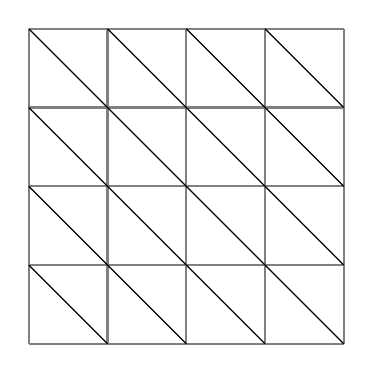
\begin{tikzpicture}
      \draw[step=1cm,gray,thick]
      (0,0) grid (4,4);

      \foreach \x in {0,...,3}{
        \draw (\x, 0) -- (0, \x) ;
        \draw (\x, 4) -- (4, \x) ;
      }

    \end{tikzpicture}
    \caption{Tri-Structured Mesh}
    \label{fig:struct}
  \end{minipage}
  \begin{minipage}{.5\textwidth}
    \centering
    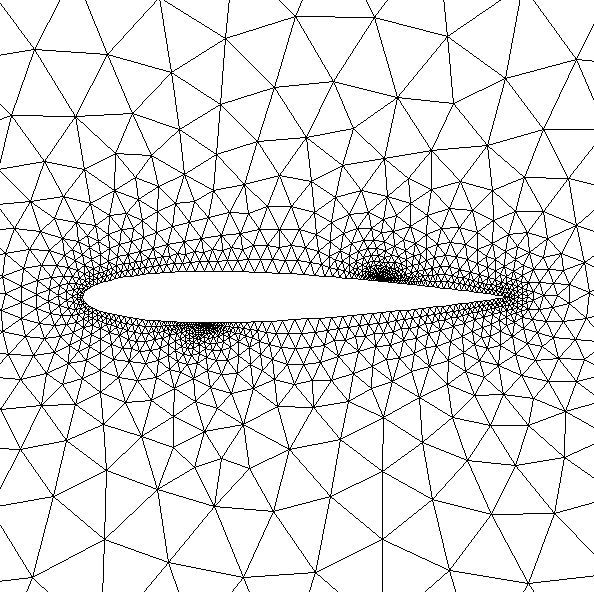
\includegraphics[width=.55\textwidth]{umesh}
    \caption{Airfoil Tri-Unstructured Mesh}
    \label{fig:umesh}
  \end{minipage}
\end{figure}
\par
\noindent A particular simulation might, for example, be approximating the velocity of a fluid in each cell, and at every time step re-calculate this value based on the values of cells around it. Programs which make use of this repeating pattern to calculate value are commonly referred to as a `stencil code' \cite{stencil}. An example of a 2D stencil is shown in Figure \ref{fig:stencil}.
\vspace{.5cm}
\begin{figure}[h!]
  \centering
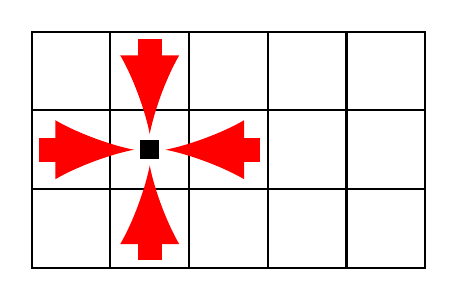
\begin{tikzpicture}

\foreach \x in {0,...,4}{
  \foreach \y in {0,...,2}{
    \node [fill=none, draw=black, thick, minimum size=1cm]
      at (\x+.5, \y+.5) {};
  }
}

\node [fill=black] at (1.5, 1.5) {};

\draw[->,>=latex, red, line width=3mm] (0.1,1.5) -- (1.3,1.5);
\draw[->,>=latex, red, line width=3mm] (2.9,1.5) -- (1.7,1.5);
\draw[->,>=latex, red, line width=3mm] (1.5,0.1) -- (1.5,1.3);
\draw[->,>=latex, red, line width=3mm] (1.5,2.9) -- (1.5,1.7);

\end{tikzpicture}
\caption{Example 2D stencil code}
\label{fig:stencil}
\end{figure}

\clearpage
\subsection{Report Structure}
The rest of this report is structured as follows: In Section \ref{s:research} (p\pageref{s:research}) the research done to inform the work in this project is discussed, along with relevant similar academic work. This is followed by a Project Specification in Section \ref{s:spec} (p\pageref{s:spec}), which includes the requirements of the project, and a high level plan of the implementation to be completed, its components, and how they will interact.
Section \ref{s:impl} (p\pageref{s:impl}) details the Implementation itself, and the expected results of code generation with JIT compilation enabled, and Section \ref{s:test} (p\pageref{s:test}) explains the plan for, and outcome of, Testing and Benchmarking using an example application on a HPC cluster.
\par Section \ref{s:eval} (p\pageref{s:eval}) contains an Evaluation of the work completed, including a discussion of Future Work (p\pageref{ss:fw}) which could build on top of what was done for this report; and a reflection on Project Management (p\pageref{ss:pm}), and lastly Section \ref{s:conc} (p\pageref{s:conc}) provides an overall Conclusion
